\documentclass[11pt, twocolumn]{article}
\usepackage[left=2.54cm, right=2.54cm, top=1.5cm]{geometry}
\usepackage{graphicx}
\usepackage{wrapfig}
\usepackage[skip=0pt, font=scriptsize,labelfont=scriptsize]{caption}
\usepackage{subcaption}
\usepackage{float}
\usepackage{hyperref}
\usepackage{amsmath}
\usepackage{mathtools}
\usepackage{siunitx}
\usepackage{textcomp}
\usepackage{gensymb}
\usepackage{color} % text color for not taking
\usepackage{pdflscape}

\graphicspath{{figures/}}

\usepackage[
backend = biber,
style=ieee,
]{biblatex}
\addbibresource{neuronNetworkReferences.bib}

\newcommand{\code}[1]{\texttt{#1}}
\DeclarePairedDelimiter\abs{\lvert}{\rvert}%

\usepackage{acro} % acronym package
\DeclareAcronym{STDP}{
	short = STDP,
	long  = Spike Time Dependent Plasticity,
}
\DeclareAcronym{MADELEINE}{
	short = MADELEINE,
	long  = 1959 seminal neural network,
}
\DeclareAcronym{CIFAR}{
	short = CIFAR,
	long  = Canadian Institute For Advanced Research,
}
\DeclareAcronym{NEURON}{
	short = NEURON,
	long  = Yale-developed neuron simulation environment,
}
\DeclareAcronym{NetPyNE}{
	short = NetPyNE,
	long  = ``Networks using Python and NEURON'' library,
}
\DeclareAcronym{PID}{
	short = PID,
	long  = Proportional Integrator Derivative (Control),
}

\begin{document}
	\begin{titlepage} 
		\newcommand{\HRule}{\rule{\linewidth}{0.5mm}} % Defines a new command for horizontal lines, change thickness here
		
		\center % Centre everything on the page
		
		%------------------------------------------------
		%	Headings
		%------------------------------------------------
		
		\textsc{\LARGE University of Sydney}\\[1.5cm] % Main heading such as the name of your university/college
		
		%\textsc{\Large Computation Neuronal Networks}\\[0.5cm] % Major heading such as course name
		
		%\textsc{\large PHYS2921}\\[0.5cm] % Minor heading such as course title
		
		%------------------------------------------------
		%	Title
		%------------------------------------------------
		
		\HRule\\[0.4cm]
		
		{\huge\bfseries Exploration of Computation Neuronal Network for Solving a Foraging Task}\\[0.4cm] % Title of your document
		
		\HRule\\[1.5cm]
		
		%------------------------------------------------
		%	Author(s)
		%------------------------------------------------
		
		%\begin{minipage}{0.4\textwidth}
		%	\begin{flushleft}
		%		\large
		%		\textit{Author}\\
		%		William .A. \textsc{Talbot} % Your name
		%	\end{flushleft}
		%\end{minipage}
		%~
		%\begin{minipage}{0.4\textwidth}
		%	\begin{flushright}
		%		\large
		%		\textit{Date}\\
		%		\textsc{} % Supervisor's name
		%	\end{flushright}
		%\end{minipage}
		
		% If you don't want a supervisor, uncomment the two lines below and comment the code above
		{\large\textit{Author}}\\
		William A. \textsc{Talbot}\\ % Your name
		{\large\textit{Supervisor}}\\
		Dr. Cliff \textsc{Kerr} % Your supervisor
		
		%------------------------------------------------
		%	Date
		%------------------------------------------------
		
		\vfill\vfill\vfill % Position the date 3/4 down the remaining page
		
		{\large May, 2019} % Date, change the \today to a set date if you want to be precise
		
		%------------------------------------------------
		%	Logo
		%------------------------------------------------
		
		%\vfill\vfill
		%\includegraphics[width=0.2\textwidth]{placeholder.jpg}\\[1cm] % Include a department/university logo - this will require the graphicx package
		
		%----------------------------------------------------------------------------------------
		
		\vfill % Push the date up 1/4 of the remaining page
		
	\end{titlepage}

\newpage
\twocolumn
%\tableofcontents

\section*{Abstract}
\textbf{Through the \acs{NetPyNE} library a simple biologically realistic spiking neural network has been created to perform a simple food-foraging task in a virtual environment. This report attempts to replicate and investigate the work by Sanda et al. \cite{sanda2017multi}, by applying reinforcement learning in the form of spike time dependent plasticity (\acs{STDP}), a simple model for how cells within the human brain are strengthened and weakened by activity. Various synaptic balancing mechanisms and strategies were imposed on the network in order to achieve double chance-level performance.}

\section*{Introduction}

\subsection*{Neuroscience and the Rise of Neural Networks}
McCulloch's and Pitt's 1943 seminal paper on the ``logical calculus'' of ``nervous activity'' \cite{mcculloch1943logical} laid the foundation for neurological modelling, leading to the first  neural network solving a real-world application, \acs{MADELEINE}, in 1959. Popular fears of artificial intelligence and robotics in the 1970's suppressing research in this area, however the mid 1980s saw a resurgence of the computational neuroscience field. Hopfield and Tank's tackling of the travelling salesman problem in 1985 \cite{hopfield1985neural} using parallel collective analog circuits is a particularly relevant example. Their electrical circuits were biologically inspired, with standard electrical components modelling the neuronal dynamics. The well-studied problem which aims to find a shortest-path circuit between points, is known to have exponential time complexity and be np-complete, however their circuit was able to produce excellent solutions in short time spans, rivalled only by the Lin-Kernighan Monte Carlo approach. The core application of neural networks was realised - ``A person ... quickly finds a very good path'' \cite{hopfield1985neural} and that therefore, conceptually at least, it should be ``an easy problem''. The question is then: why can the brain quickly solve computationally difficult problems with relative ease, and is this replicable? 

Advances in robotics, and perceptual, pattern-intensive and data-dependent problems \cite{hopfield1985neural} are ongoing today. Today many network models exist, such as feed-forward, recurrent, bi-directional recurrent, biological, spiking, convolutional, max-pooling convolutional, deep belief, self-delimiting and time delay neural networks \cite{schmidhuber2015deep}. Object classification is an example of a widely developed subset of neural net applications, however even today the best performances of these networks are sub-human and sometimes significantly worse. One recent convolutional neural network developed by Liang and Hu \cite{liang2015recurrent} trained on 50000 images of the 10-class \acs{CIFAR}-10 database achieved accuracies of less than 93\% while another, trained on 60000 images of the 100-class \acs{CIFAR}-100 database has a best accuracy of only 68.25\%. 

Noticeably most modern neural network development has diverged from neuroscience due in part to the complexity of brain biology, however not only is the accuracy of current artificial neural networks inferior to the human brain but also the size of the training set required to teach a neural network is disproportionately large comparatively. The potential for networks that require much smaller training sets is a motivator for investigating biologically realistic neural networks. So far despite their computationally feasibility \cite{zenke2014limits}, spiking neural networks have shown lessened learning capabilities compared to the best traditional neural networks \cite{schmidhuber2015deep}. Some biologically realistic neuron network projects are ongoing today however \cite{ashby2011tutorial}\cite{ashby2005frost}\cite{frank2005dynamic}\cite{hartley2006understanding}\cite{leveille2010running}, including the Human Brain Project \cite{markram2015reconstruction}, who develop a ``unified infrastructure for computational neuroscience'', and ``BioSpawn'' \cite{eliasmith2016biospaun}, a dynamic brain simulation consisting of 2.5 million neurons in visual, motor and memory populations. Even physical neuron networks have been demonstrated \cite{frega2014network}, providing further avenues for the field.

The complex systems lab at the University of Sydney has also made significant developments in the field's digital side, with sensorimotor cortex models able to demonstrate reinforcement learning through spike time dependent plasticity (\acs{STDP}) in a virtual arm \cite{neymotin2013reinforcement}\cite{dura2017evolutionary}. Sanda et al.'s team at the University of California have similarly demonstrated effective \acs{STDP} reinforcement learning within a toy game, similar computationally to the travelling salesman problem \cite{sanda2017multi}. This report will demonstrate an implementation of Sanda et al.'s network and investigate the effects of modifications to the network. \acs{NetPyNE}, a tool for creating and running large-scale network simulations in \acs{NEURON} \cite{dura2018netpyne} was used as the fundamental neuron simulation environment.

\subsection*{Understanding Neurons and Spiking Neural Networks}

\begin{figure}[H]
	\centering
	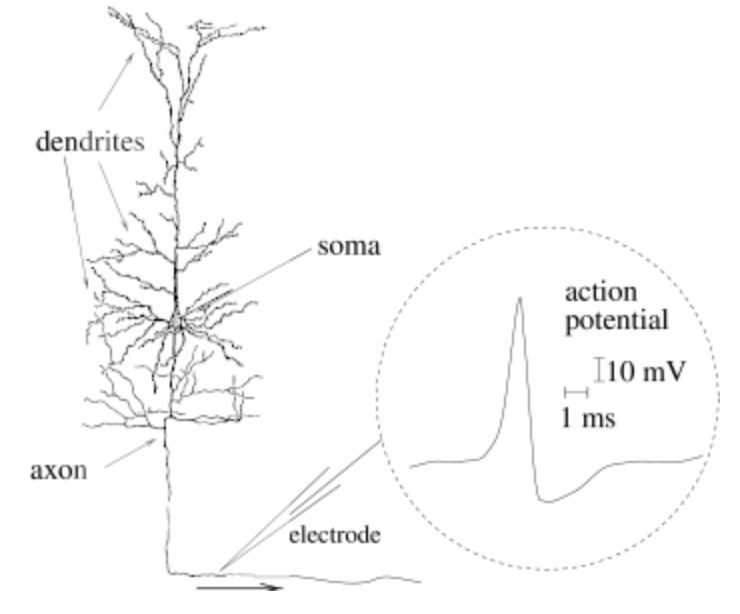
\includegraphics[width=\linewidth]{neuron_diagram}
	\caption{Neuron Diagram \cite{gerstner2014neuronal}}
	\label{fig:neuron_diagram}
\end{figure}

Modern biologically realistic neuron models provide the foundation for the software implemented in this project and so this report will provide an introduction to neuronal dynamics sourced primarily from the \textit{Neuronal Dynamics} textbook \cite{gerstner2014neuronal}. The simple neuron consists of a central nucleus, the``soma'', which acts as the non-linear processing unit of the cell, ``dendrites'', into which electric signals enter the cell, and the ``axon'' which is the output device of the cell. ``Synapses'' are the biological interface between dendrites and axons and many types exist which enables neurons to have different electrical characteristics. Neurons belong to populations of like neurons and often exist in layers, such as the cortex tissue, approximately 3 millimetres deep on the outer surface of the cerebellum, where much sensory, motor and association processes occur.

The basic unit of signal transmission is the ``action potential'', a sharp voltage spike with a magnitude of approximately 100mV and typical duration of 1-2 milliseconds. When many spikes arrive at a soma from its dendrites, they accumulate and when the potential of the cell is high enough the neuron will produce an action potential of its own which travels along its axon to dendrites of other neurons. It is these through these signals that communication occurs between neurons and sophisticated behaviour is able to emerge. Gradually models have been developed to model the electrical characteristics of various neurons and the most prevalent is the Integrate-and-Fire models. In the simplistic ``Leaky'' Integrate-and-Fire model, input is linearly integrated - the cell's potential $u(t)$ (also called ``membrane potential'') is described by a linear differential equation which decays with some time constant $\tau$ and resets to 0 if it passes a threshold value $\vartheta$. This mathematical model can be simplified further by treating the action potential spikes as Dirac-delta pulses.
\begin{equation}
	\tau\frac{du}{dt} = -[u(t)-u_r]+RI(t)
	\label{eqn:leaky_integrate_and_fire_differential}
\end{equation}
%\vspace{-10mm}
\begin{equation}
	\text{if } u(t) > \vartheta \text{ then } \lim\limits_{\delta\leftarrow0;\delta>0}u(t+\delta) = u_r
	\label{eqn:leaky_integrate_and_fire_threshold}
\end{equation}

More sophisticated non-linear models (``Generalised'' Integrate-and-Fire models), have been developed based on the empirical biophysical properties of neurons. The first was the Hodgkin-Huxley model of a giant squid's neuron in the 1950s, and since then neuroscientists have discovered hundreds of types of ion channels and this rich biophysics leads to much nuance in neuron electrical behaviour. This includes hyper-polarisation of the cell and refractory periods of suppressed firing, spike-frequency adaptation, sub-threshold effects and post-inhibitory rebound. Exponential and quadratic Integrate-and-Fire models with adaptation and stochastic variables are some examples of non-linear models that have been reasonably fit to experimental data. When these models are used for their appropriate class of simulated neurons, we are able to generate networks that exhibit biologically realistic behaviour. 

It is important to introduce the concept of inhibition in neuronal networks. Inhibitory neurons, unlike excitatory neurons discussed so far, produce action potentials that decrease the membrane potential of the receiving neuron rather than increase it, reducing it further below its firing threshold and have ``inhibits'' firing. Inhibitory neurons maintain balance in a network, preventing it from becoming over-stimulated or ``epileptic''. Populations of excitatory and inhibitory neurons together can form useful spiking neural networks.

The final major component of the neural network model is how it is able to be modified over time. The approach taken is reinforcement learning through spike time dependent plasticity (\acs{STDP}). \acs{STDP} increases of the strength of a connection if the input, or pre-synaptic spike to a neuron is followed by a post-synaptic spike, also called a ``pre before post'' event \cite{sanda2017multi}. In unsupervised \acs{STDP}, whenever this occurs the connection between the respective neurons is increased, and conversely if a ``post before pre'' event occurs the connection is weakened. This report will utilise a form of reinforcement learning \acs{STDP} mechanism, whereby the strengthening or weakening of a connection that experienced a \acs{STDP} event is delayed and the selection of reward or punishment is chosen at regular intervals depending on performance.

\section*{Methods}

\subsection*{The Foraging Problem and Network Structure}
The details of the foraging problem are almost identical to that of Sanda et al.'s implementation \cite{sanda2017multi}, in which ``epochs'' of 300 milliseconds divide up the simulation with a 0.5 ms integration time-step. The virtual environment was composed of a 49x49 occupancy grid containing  randomly-scattered food with density 0.1. At the end of each epoch, the virtual sprite moved one square in one of the eight compass directions and if any food occupied that square, it was ``gathered'' and another was placed randomly in the environment to maintain constant density. Each epoch lasted long enough for the neural network to receive input stimuli, process this stimuli and produce an output. The neural network itself contained three layers of Izhikevich regular spiking pyramidal cell neurons \cite{izhikevich2007dynamical}\cite{izhikevich2008large}; an 7x7 input layer (I), a 28x28 middle layer (M) and 3 by 3 output layer (O). 

\vspace{-3mm}
\begin{figure}[H]
	\centering
	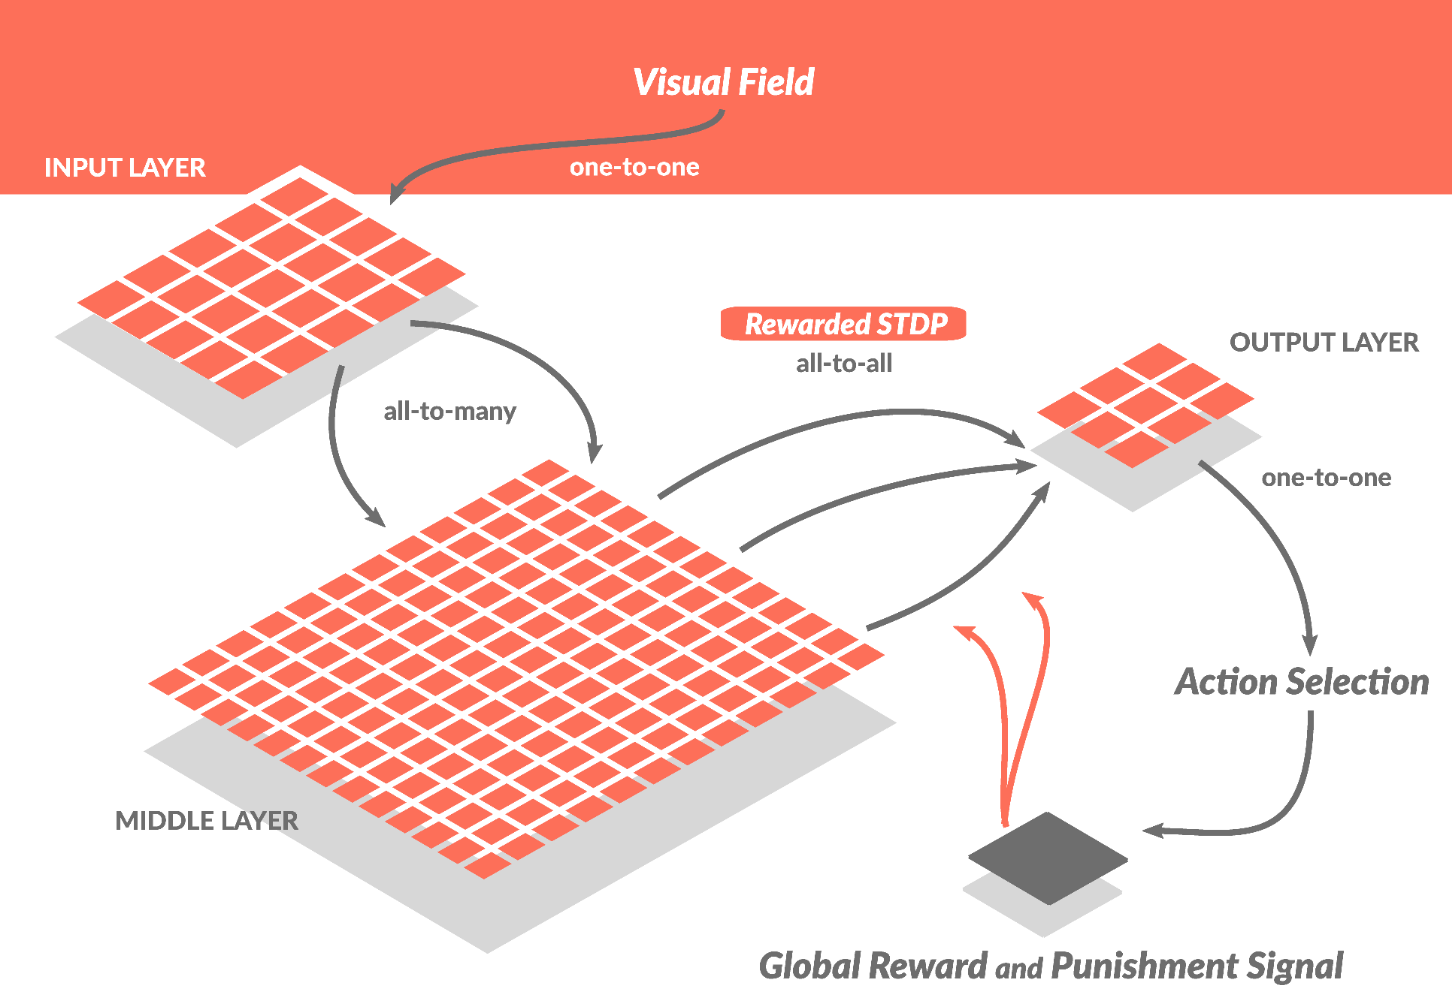
\includegraphics[width=\linewidth]{layers_diagram}
	\caption{Diagram of Input, Middle and Output Layer Inter-Activity \cite{sanda2017multi}}
	\label{fig:layers_diagram}
\end{figure}
\begin{figure}[H]
	\centering
	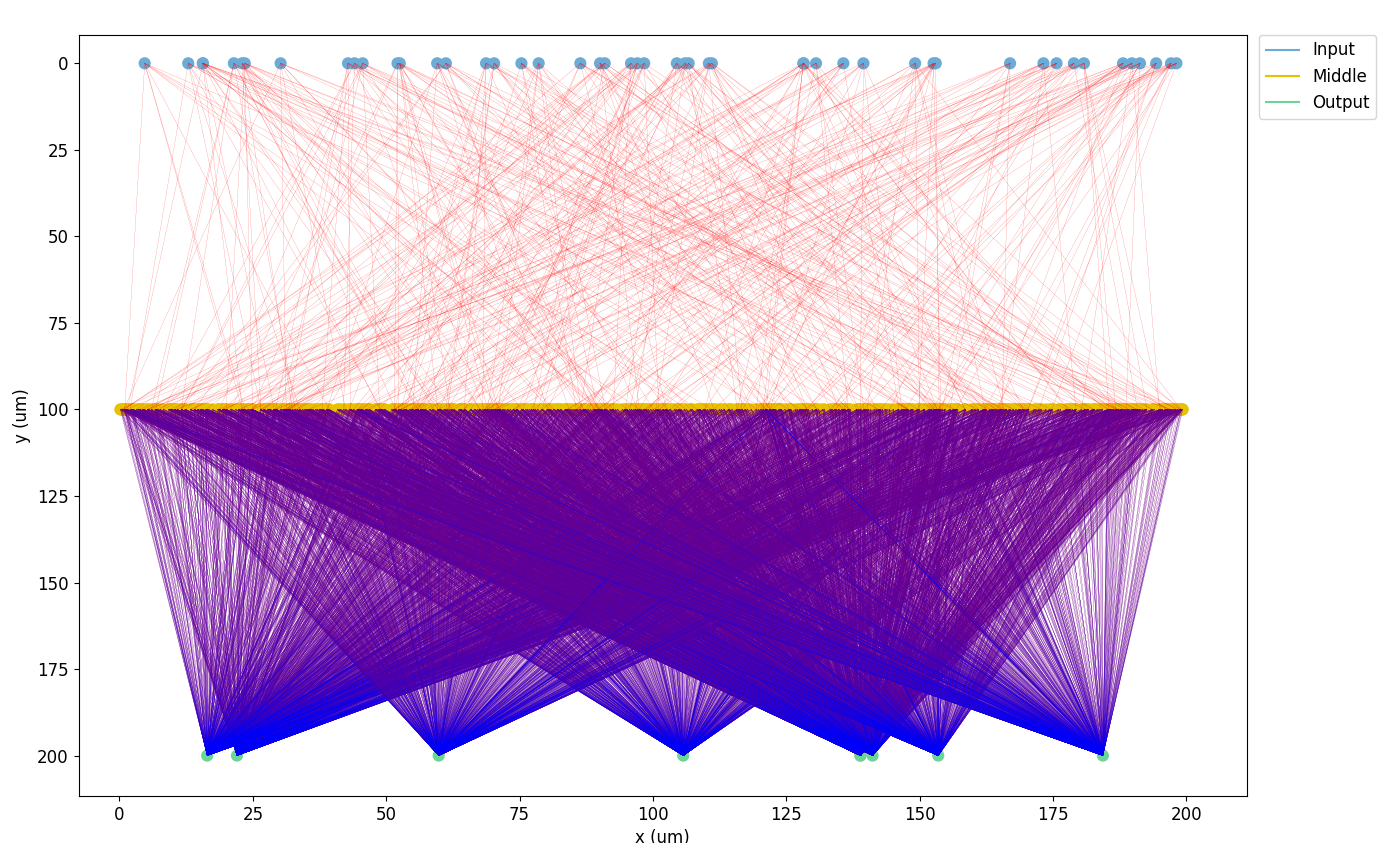
\includegraphics[width=\linewidth]{network_connections}
	\caption{Diagram of Connections between Input, Middle and Output Layers}
	\label{fig:network_connections}
\end{figure}

The input layer which provided the only stimulus to the network is related to the 7x7 ``visible'' area around the sprite, such that only the neurons in this layer that corresponded to a food-occupied grid location were stimulated at each epoch. Hence 8 neurons of the layer corresponded to the inner circle around the sprite, 16 corresponded to one move further out and 24 corresponded to the outermost circle of occupancy in the visual field of the sprite. the ``middle'' neuron  of this layer corresponding to the sprite was never stimulated. Each input layer neuron had uniform weight excitatory connections to 9 randomly selected middle layer neurons, and each of these middle layer neurons were connected to every output layer neuron with initial weights drawn from a normal distribution. The output neurons each correspond to a compass direction except the middle and whichever spiked most was used as the direction Pseudo-random numbers were generated to break ties. Additionally to prevent movement cycles in the learning process, there was a 1\% chance for a random direction to be chosen.

\subsection*{Implementing \acs{STDP}}
Rewarded spike time dependent plasticity (\acs{STDP}) was implemented between the middle layer neurons and output neurons such that at the end of each epoch, the sprite moved and if food was gathered then the synaptic connections which had experienced ``pre before post'' activity were strengthened. If food was not gathered, then these connections were weakened, however since this outcome is likelier, punishment was set to be -0.1 times that of the reward. The model for \acs{STDP} was taken from a model of reinforcement learning for a two-joint virtual arm \cite{neymotin2013reinforcement} \cite{chadderdon2012reinforcement}, as was the algorithmic structure of fixed frequency update calls within the NetPyNE simulation. However \acs{STDP} alone is insufficient to train a network, and so synaptic balancing mechanisms, random variability and inhibition were used in order to obtain above-chance level results.

\subsection*{Synaptic Balancing Mechanisms}
In total four synaptic balancing mechanisms were used to obtain above-chance gathering rate performance. Without any of them the network tended to some extreme of synaptic activity that did not allow for learning to occur.

\subsubsection*{1. Hetero-synaptic Balancing}
In both experimental studies and detailed biological models it has been shown that the sum of input synapse weights to any cell must be held approximately constant to prevent runaway spiking dynamics \cite{sanda2017multi}. Therefore a simple rule was implemented such that whenever a single input synapse's weight was adjusted by the \acs{STDP} mechanism, all other input synapses were adjusted to compensate and thus constant synaptic input to each cell was maintained. Due to the implementation of frequency targeting, this constant synaptic input is in fact a very slowly changing variable that depends on the firing frequencies of the output neurons.

\subsubsection*{2. Frequency Targeting}
It was found that the spiking frequency of the output neurons was crucial for decision making \cite{sanda2017multi}. When spiking frequency of the output layer was low ($<1$ Hz), the number of silent epochs (zero spikes) were high as excitability was insufficient to reach the spiking threshold. Increasing the output layer excitability prevent long lengths of silent output epochs however increasing it too much resulted in epochs where all the output cells spiked, and some multiple times, thus increasing the number of non-zero ties. A frequency of 1.6 Hz was chosen as a default output firing rate as a good balancing point between silent epochs and high-spiking spike-tied epochs. To achieve this desired frequency, the excitatory weight sum was gradually adjusted using a slow-moving variable that represented the target synaptic weight $W_T$ of the cell. If the particular output cell was firing under the desired frequency, this variable was increased and if it was over-firing this variable was decreased by $\Delta_W$ as per equation \ref{eqn:frequency_targeting}. This served as a weak proportional controller.
\begin{equation}
	W_T(n+1) =
	\begin{cases} 
	W_T(n)\cdot(1+\Delta_W) & f_{spike} < f_{target} \\
	W_T(n)\cdot(1-\Delta_W) & f_{spike} > f_{target}
	\end{cases}
	\label{eqn:frequency_targeting}
\end{equation}

\subsubsection*{3. Output Balancing}
Previous work by the authors of the modelled paper revealed that balancing the weights of output synapses helped prevent a several neurons controlling the whole network and others from dying off entirely \cite{skorheim2014spiking}. This was implemented by dividing the \acs{STDP} reward by a normalising ratio $R_n$, equal to the current synaptic output sum divided by the initial synaptic output sum for each cell (equation \ref{eqn:output_balancing}).
\begin{equation}
	R_n = \frac{\sum W_{curr}}{\sum W_{init}}
	\label{eqn:output_balancing}
\end{equation}
As a result already strengthened neurons were less able to increase in weight compared to weaker neurons, advantaging them over the already dominating neurons.

\subsubsection*{4. Soft Thresholding}
The final synaptic balancing is a method called ``soft thresholding'' which was an option of the \acs{STDP} model used. This mechanism is similar to output balancing in that it adds another multiplicative factor to the synaptic reward or punishment that depends not on any other synaptic connection weights but on a chosen maximum weight. As the synaptic weight increases towards this value, this ratio $S$ for positive rewards approaches 0 and 1 for punishments as per equation \ref{eqn:soft_thresholding}. As the weight decreases towards zero, the inverse of this relation is true, and so no weight can ever reach 0 or the maximum (set to 10 times the average starting excitatory weight) by the \acs{STDP} mechanism.
\begin{equation}
	S = \quad
	\begin{cases} 
	\left(1-\frac{W}{W_{max}}\right) & \text{ if rewarding} \\
	\frac{W}{W_{max}} & \text{if punishing}
	\end{cases}
	\label{eqn:soft_thresholding}
\end{equation}


\subsection*{Random Variability}
Noise and random variability is an omnipresent component of almost any neural network and allows random outputs to occur for a given input, which may or may not be rewarded. If this is able to occur in some way several times then it is likely that the synapse's strength will surpass its peers and if ``correct'' is much more likely to strengthen further, while if not, is likely to fall in strength back to average or lower. Random variability was introduced into the system in several ways. The initial weights of the excitatory connections were drawn from the absolute value of a normal distribution with 0.5\% variance. Additionally the planar coordinates of each layer ($x$ and $z$ coordinates) were drawn from a uniformly random distribution within a fixed square and the layers separated along the $y$ axis by 100 $\micro$m. The action potentials travelled between connected neurons with a propagation velocity of 100 $\micro$m/ms and thus a random geometrical arrangement enabled variability in the arrival of action potential signals.

\subsection*{Inhibition}
A simple inhibition model was used in this simulation based on the model employed by Sanda et al. \cite{sanda2017multi} whereby each excitatory connection between the middle and output layers was paired with an inhibitory connection with roughly the same net weight which was essential in preventing over-stimulation of the output layer. It was essential that the weight of the inhibitory connections was carefully tuned to be under the net final excitatory weight since over-inhibition led to silent epochs while under-inhibition achieved epochs with many non-zero ties. \acs{NetPyNE} is very capable of creating populations of inhibitory neurons and implementing a middle layer with mixed excitatory and inhibitory neurons would be of interest for further study as a more biologically realistic neuronal network model.

\section*{Results}
The holy grail for this project was to be able to achieve results close to those published by Sanda et al. \cite{sanda2017multi} in their 2017 paper, who managed to achieve gathering rates of 52\% under standard density conditions. This is compared to some heuristic algorithms which could achieve a gathering rate of 56\%. Since the problem is np-hard, there is no known polynomial time algorithm that solves this problem and thus no know upper efficiency limit. Therefore heuristics like this can serve as a reference point for what is close to optimal. Figure \ref{fig:random_movement} shows the performance of a system moving purely randomly and allows us to benchmark chance-level performance at 0.05. This number is logically sound too, since although the density is 0.1, we would expect to return back to visited locations just as often as moving to new locations. Since it is possible for the network to get locked in movement loops, chance level performance for a non-learning network may fall below this. 

\begin{figure}[H]
	\centering
	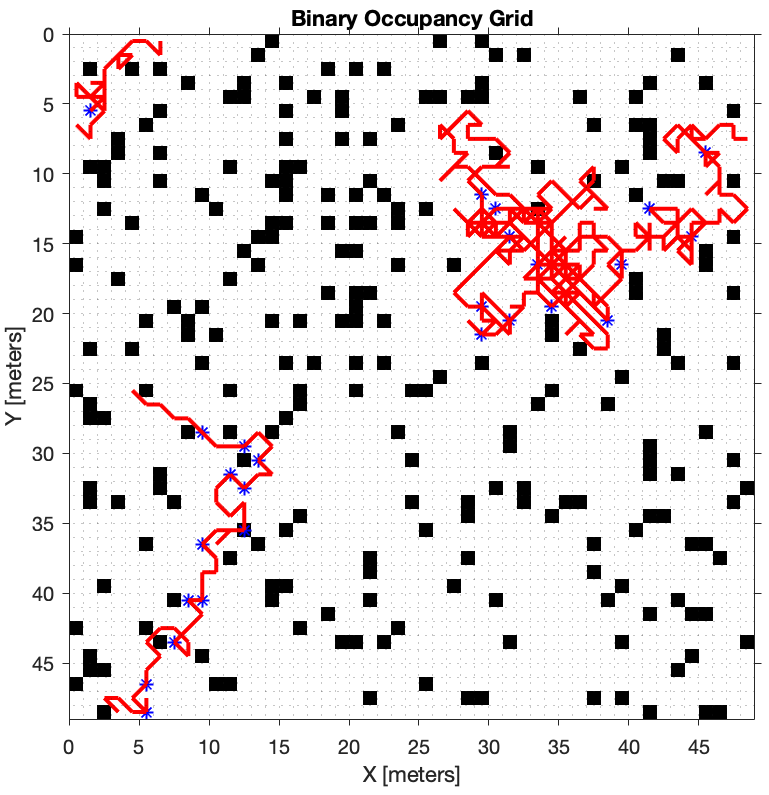
\includegraphics[width=\linewidth]{learned_path}
	\caption{Example Path After Learning (red is path, blue is collected food, black is uncollected food)}
	\label{fig:learned_path}
\end{figure}

Various simulations were conducted with maximum performance of 0.100, double chance-level, achieved by one of the two $250\times10^3$ epoch simulations, which took approximately 40 hours to run. The other yielded a performance of approximately 0.095. One further 97 hour simulation was run with $500\times10^3$ epochs that yielded a final performance of almost 0.08. While these results are significantly below the 0.56 target, they were certainly above chance level. Figure \ref{fig:performance_500k} illustrates the changing performance of the network over the $500\times10^3$ epoch simulation and like the shorter simulations, the network is able to reach its peak performance at around the 100000$^{th}$ epoch before stabilising. \ref{fig:performance_improvements} shows potential performance improvements above 0.1 when the soft-thresholding cap was increased, however time constraints in the project limit these investigations to future work.

\begin{figure}[H]
	\centering
	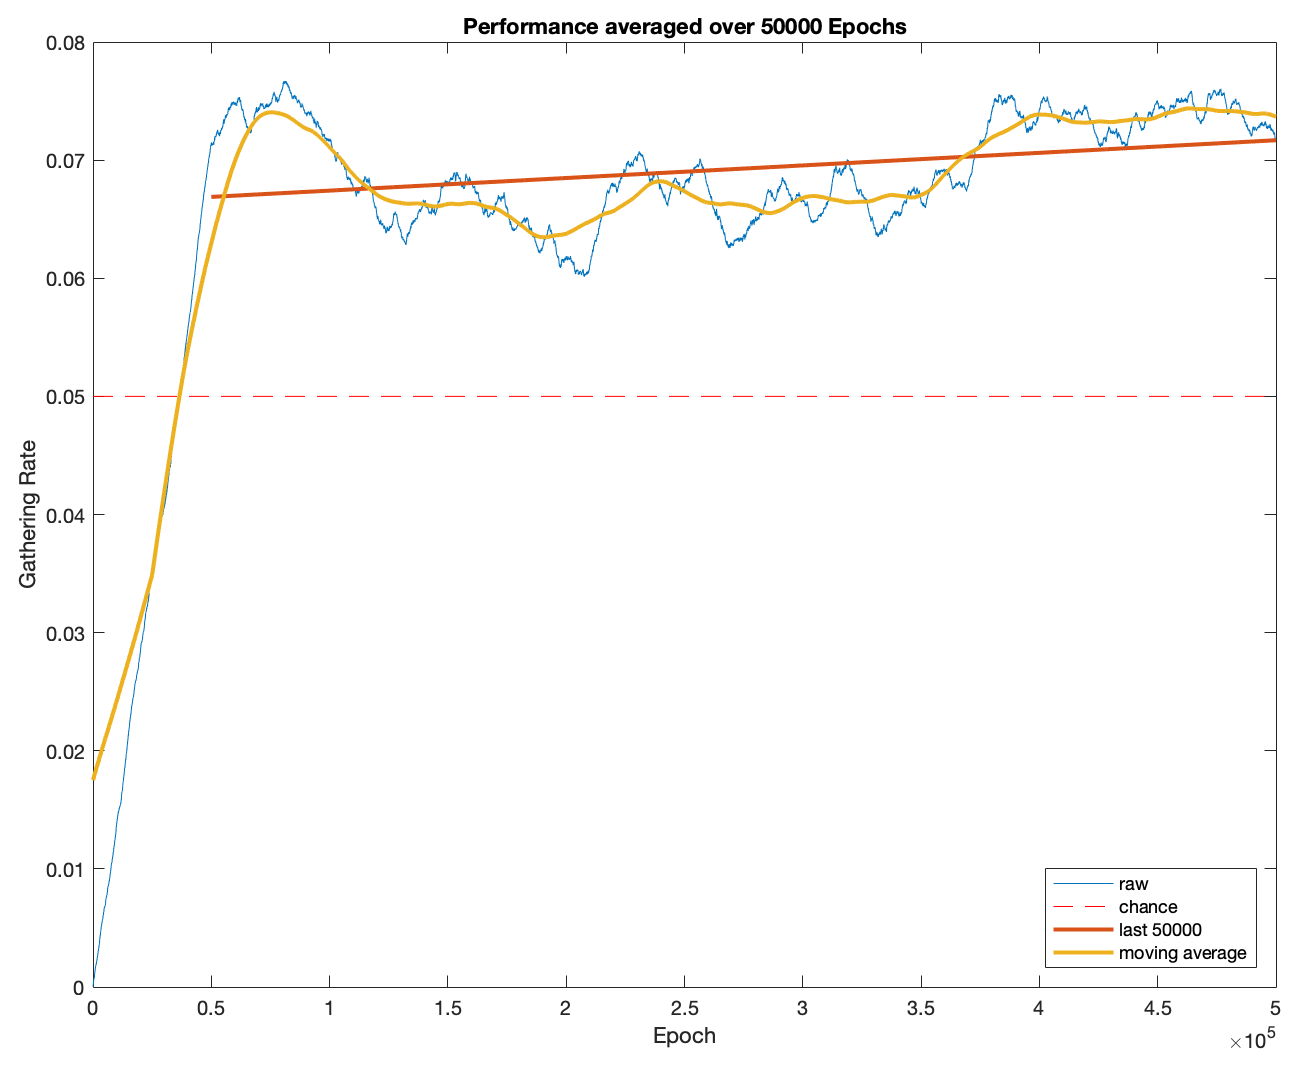
\includegraphics[width=\linewidth]{performance_500k}
	\caption{Performance Characteristics Over $500\times10^3$ epochs}
	\label{fig:performance_500k}
\end{figure}

\section*{Discussion}
While the raw performance failed to match that of the paper it was based on, all simulations longer than $100\times10^3$ epochs showed performance above chance level, and interestingly many expected characteristics of a working network were observed. One observation was the divergence of synaptic weights seen in figure \ref{fig:weights_drift_2D}, where some synapses die off immediately while a separate group diverges away and settles with a normal distribution among its weights. The same was observed by Sanda et al. \cite{sanda2017multi}, and we can see from figure \ref{fig:weights_drift_3D} that this is achieved before $100\times10^3$ epochs have passed. We expect punishment from rewarded \acs{STDP} and hetero-synaptic plasticity to kill off any unwanted synapses while the soft-thresholding restricts the synaptic weights proportional to a maximum weight. It may be possible that the combinations of balancing mechanisms to this synaptic group is too restrictive and limits the learning capabilities of the network too much. We can also visualise these synaptic weights as a heatmap and compare the initial normally distributed weights to the final separated distribution (figures \ref{fig:final_synapse_weights} and \ref{fig:initial_synapse_weights}).
\begin{figure}[H]
	\centering
	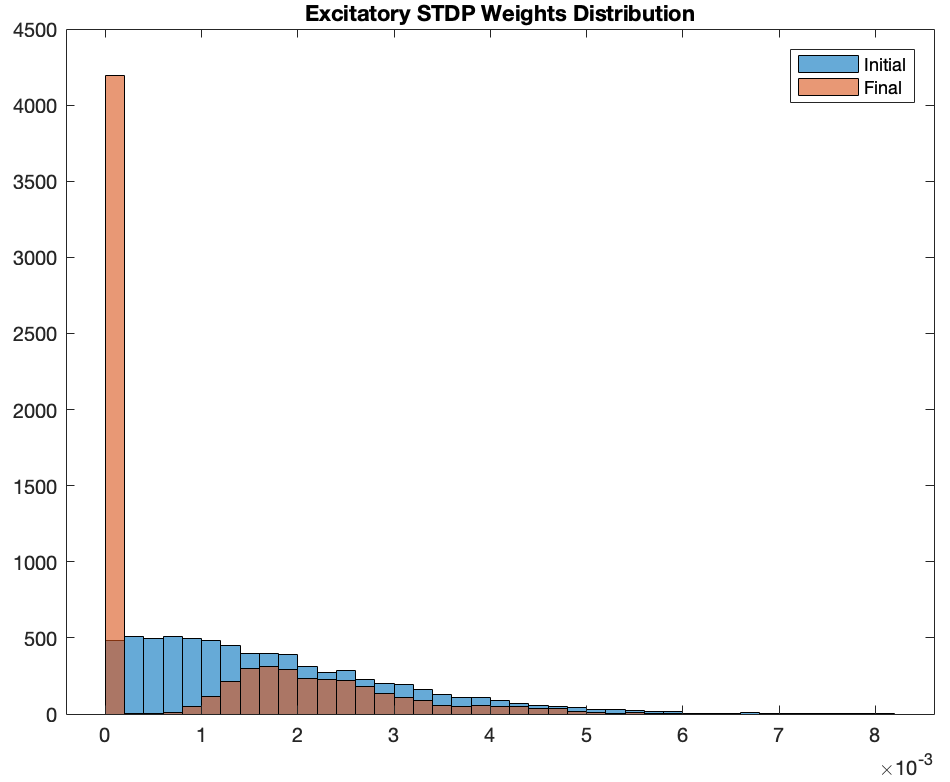
\includegraphics[width=\linewidth]{weights_drift_2D}
	\caption{Divergence of a group of excitatory synapses to a distribution}
	\label{fig:weights_drift_2D}
\end{figure}

Additionally we observe that the spiking characteristics of the epochs is approximately normally distributed, as was found by Sanda et al. \cite{sanda2017multi} when the activity of the output layer was at is right excitability. This is shown in figure \ref{fig:spikes_per_epoch}, and the additional zeros can be attributed to the ``warming up'' period of the network when excitation and inhibition are not yet balanced.

\begin{figure}[H]
	\centering
	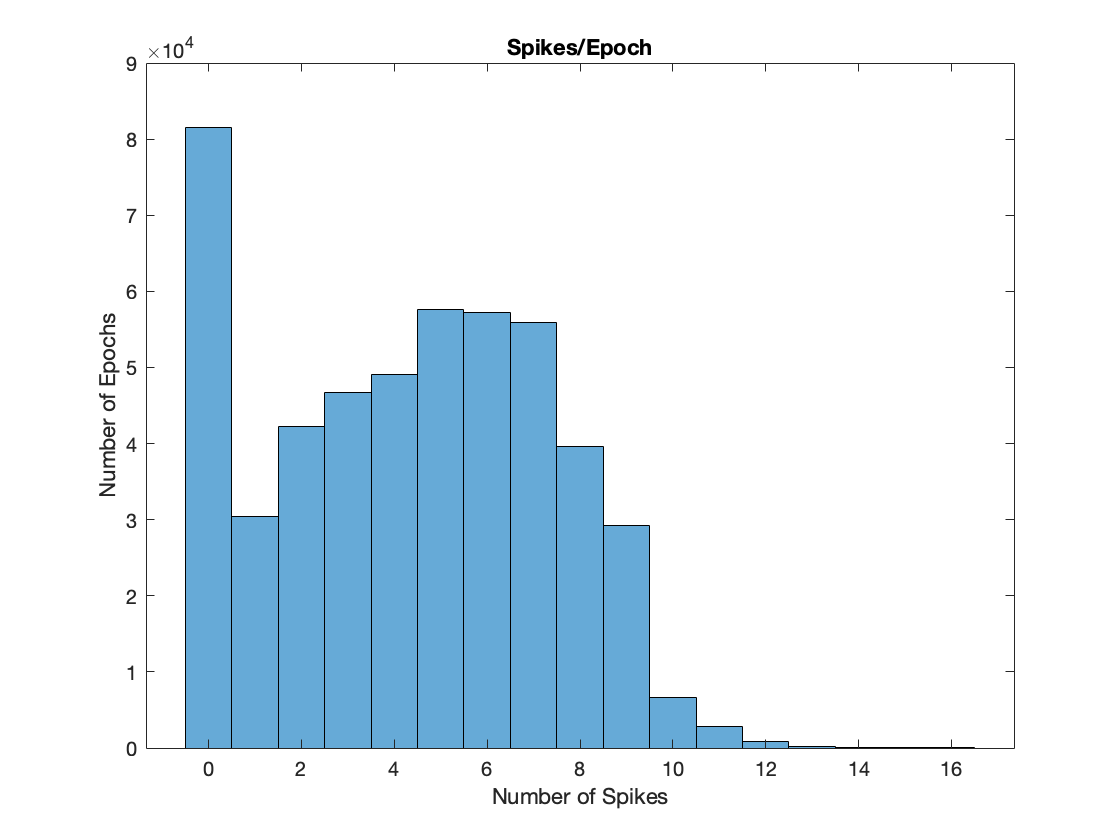
\includegraphics[width=\linewidth]{spikes_per_epoch}
	\caption{Spikes Per Epoch Histogram}
	\label{fig:spikes_per_epoch}
\end{figure}

Finally we are able to validate that as per the frequency balancing synaptic mechanism the output frequencies of the output cells remain at a constant 1.6 Hz target, as shown in figure \ref{fig:output_cell_freqs}.

\begin{figure}[H]
	\centering
	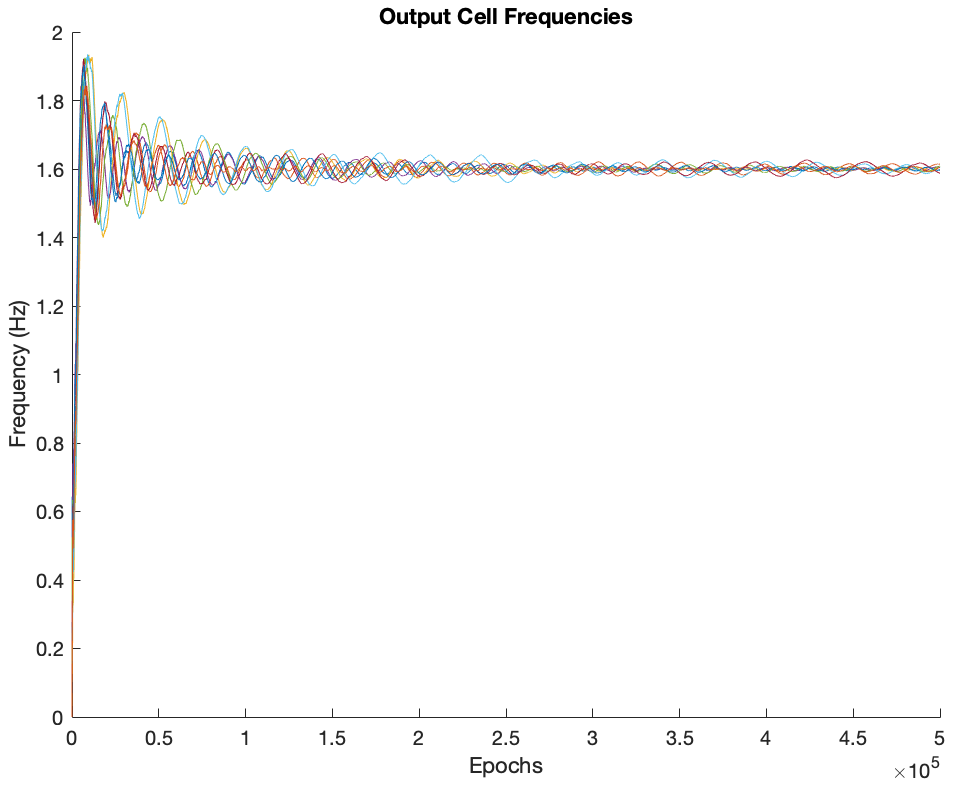
\includegraphics[width=\linewidth]{output_cell_freqs}
	\caption{Output Cell Frequencies (Hz)}
	\label{fig:output_cell_freqs}
\end{figure}
The oscillations observed in the early epochs arise because the target synapse inputs $W_T$ are offset from the required synapse inputs to achieve the desired 1.6 Hz frequency target. To compensate, this variable is changed very gradually and the frequency of the output cells lags behind this value. When the output cell frequency reaches its desired level, the slow-moving variable will have overshot the target, and so the process reverses. There are many known techniques in control theory that would be able to improve the characteristics of this output frequency response such as decrease settling time and overshoot, such as a \acs{PID} (proportional-integrator-derivative) controller. This was not deemed necessary at this stage in this project as the frequencies reached acceptable levels of within 20\% of the target by $20\times10^3$ epochs.

\section*{Conclusion}
Despite time limitations incurred by simulation time this report is able to demonstrate a partial validation of the Sanda et al. \cite{sanda2017multi} food-foraging neural network and leaves many avenues open for future work. The failure of the network to reach close to the 0.56 heuristic algorithm or Sanda et al.'s 0.51 indicates that there is still potential for investigation into how the synaptic balancing mechanisms interact and why some mechanisms limit the network's learning above a certain threshold. Synaptic noise and normalisation of synaptic potentiation around the network average are two additional components of Sanda et al.'s network that could be implemented in later work. Furthermore middle layer interconnectivity, biologically realistic inhibitory neurons and modifying the physical 3D geometry of the network are just some of the many ways in which the system could be made more biologically realistic. Despite this, it has been demonstrated that rewarded \acs{STDP} in a regulated network is capable of producing learning outcomes for a simple foraging task.

\printbibliography{}

\newpage
\section*{Contribution and Reflection}
This report and code implementation was conducted by William Talbot over the course of the semester using the \acs{NetPyNE} library based on \acs{NEURON}. While no code was available from the \textit{Multi-Layer network utilizing rewarded spike time dependent plasticity to learn a foraging task} paper \cite{sanda2017multi} that was the basis of this report, this paper provided invaluable insights into the neuronal mechanisms needed to regulate activity with neuron populations and without which this report would not exist. I would like to thank my supervisor Dr. Cliff Kerr for his help and patience while I was learning the basics of neuroscience \cite{gerstner2014neuronal} and for his assistance in building my first non-epileptic network. This has been a captivating project combining modern Neuroscience with cutting edge simulation software and machine learning theory, and a thoroughly rewarding experience.

\printacronyms[name=Acronyms]

\section*{Supporting Figures}
\begin{figure}[H]
	\centering
	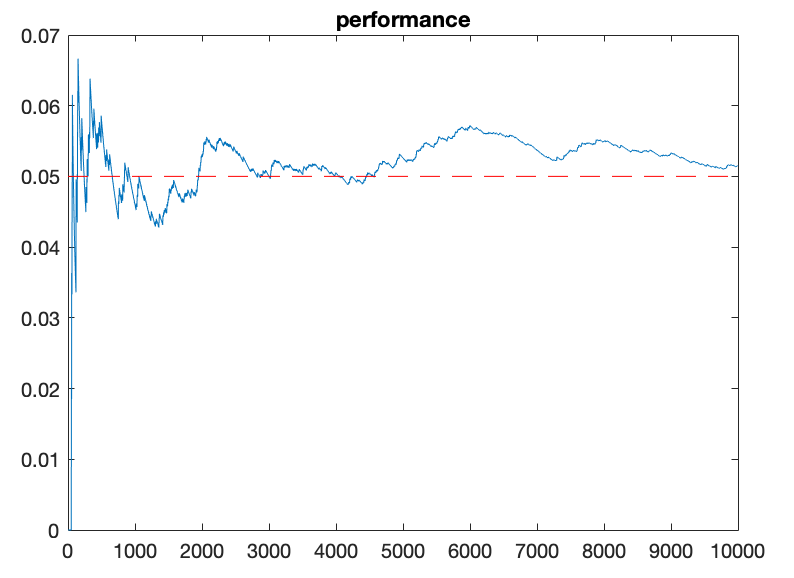
\includegraphics[width=\linewidth]{random_performance}
	\caption{Random Performance}
	\label{fig:random_movement}
\end{figure}

\begin{figure}[H]
	\centering
	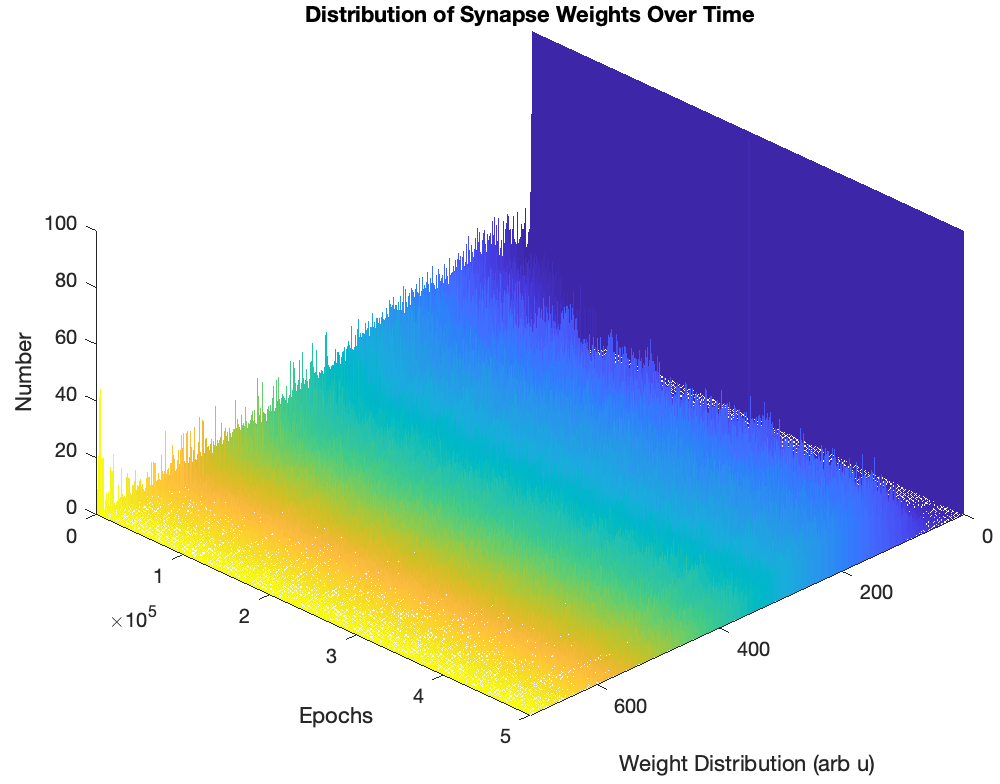
\includegraphics[width=\linewidth]{weights_drift_3D}
	\caption{Divergence of a group of excitatory synapses to a distribution over all epochs}
	\label{fig:weights_drift_3D}
\end{figure}

\begin{figure}[H]
	\centering
	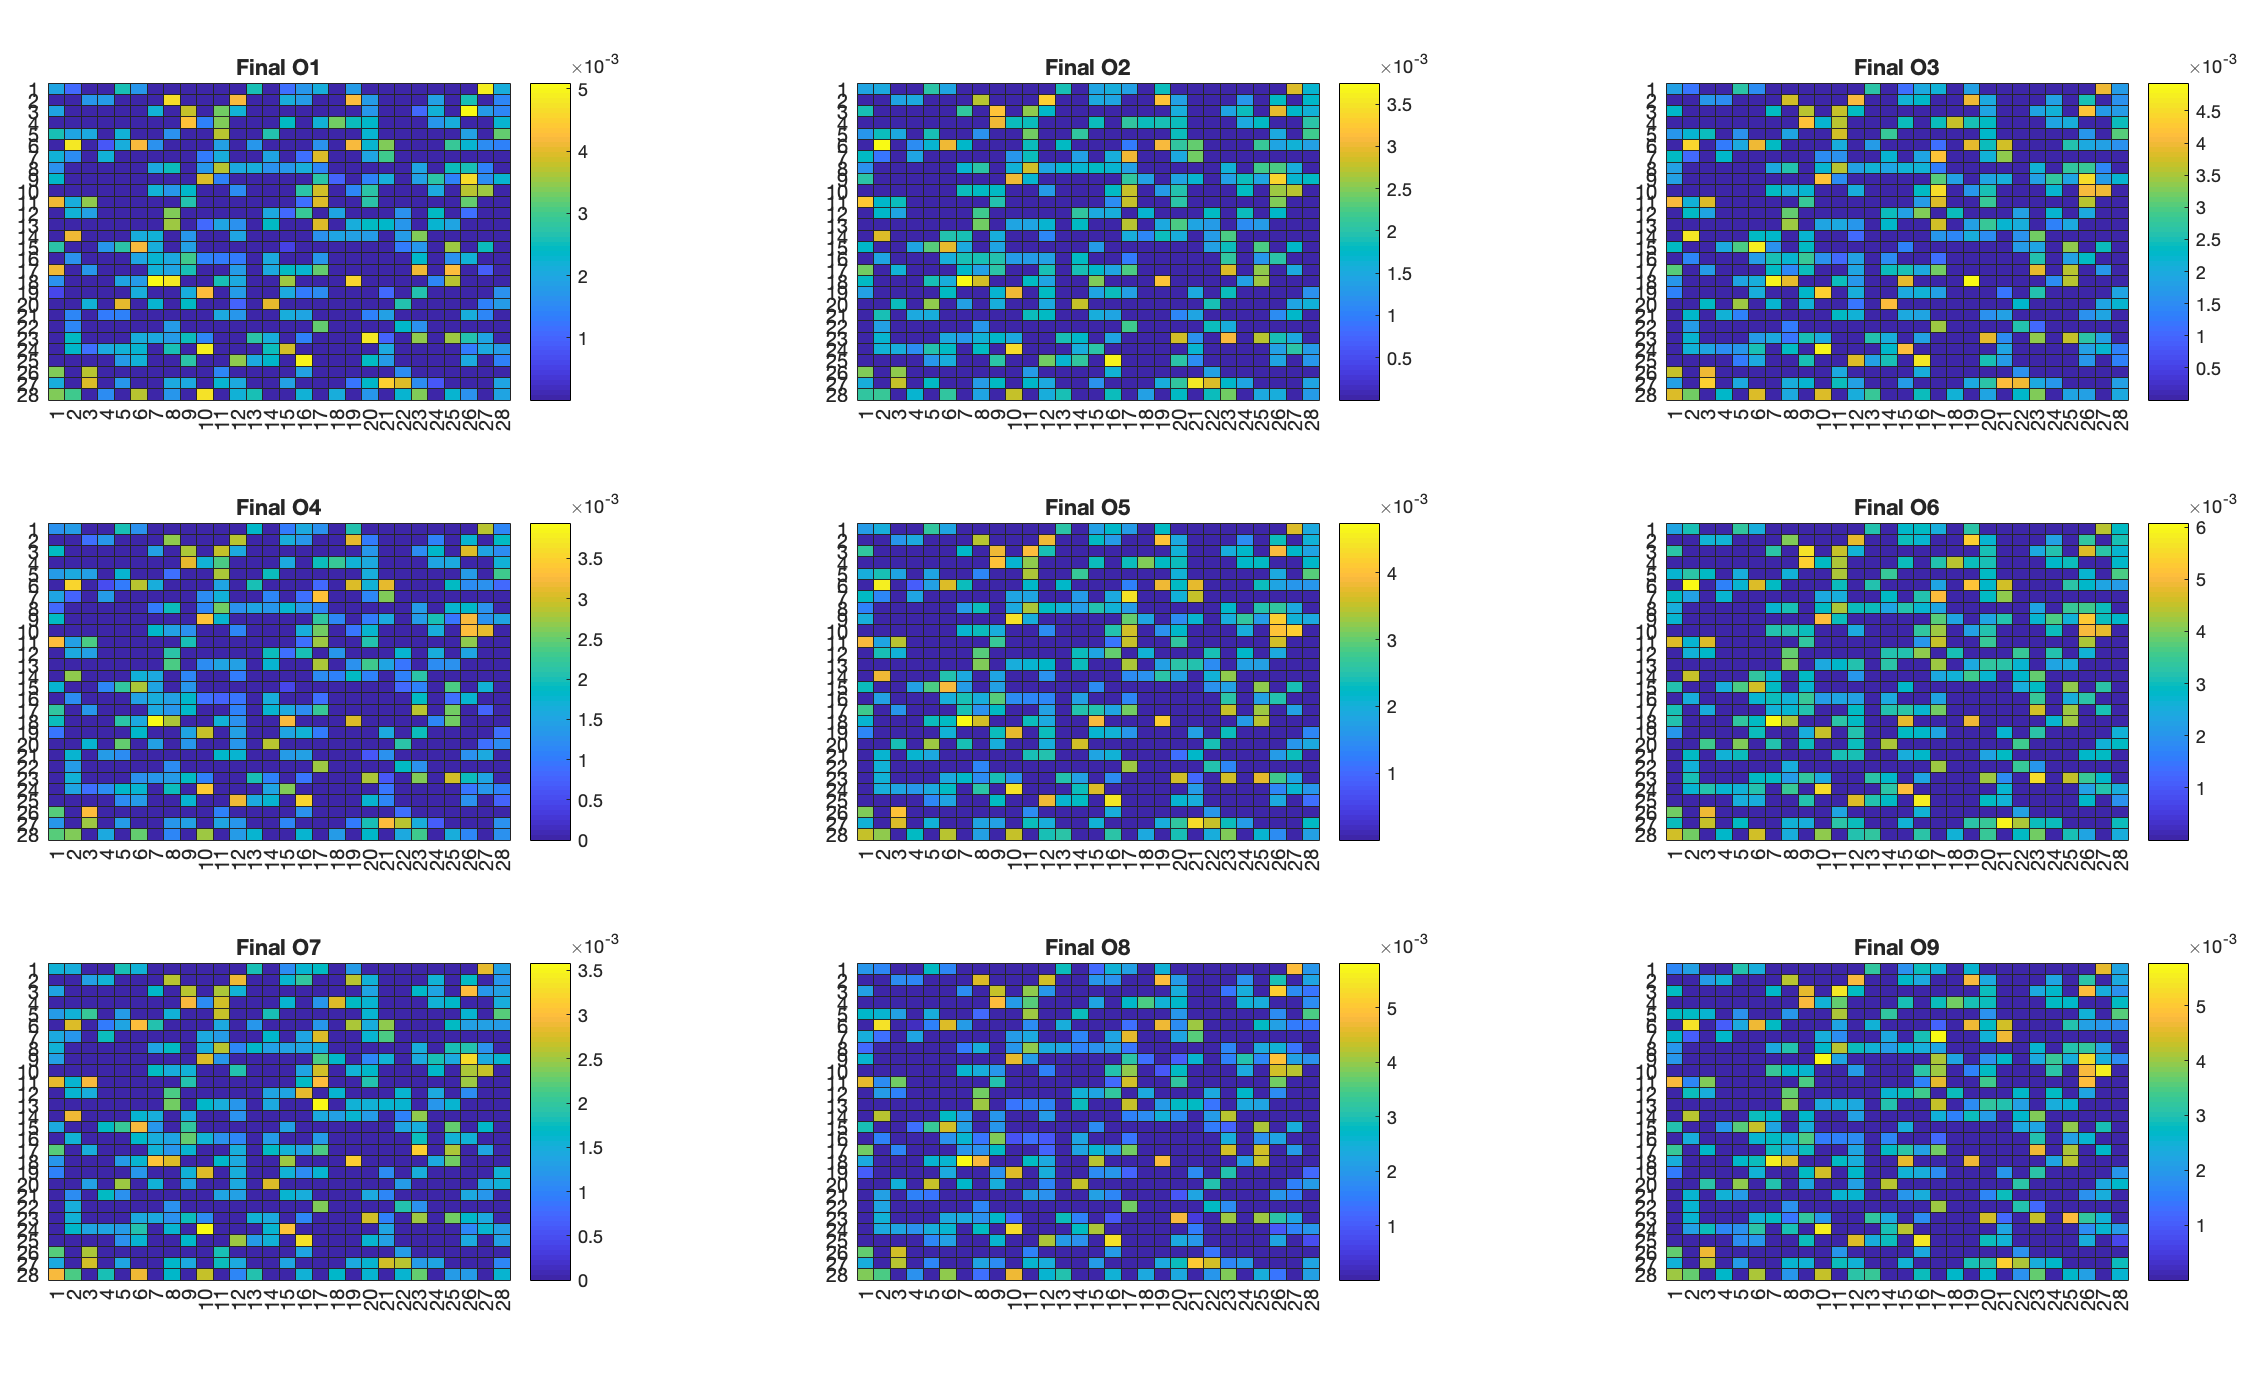
\includegraphics[width=\linewidth]{final_synapse_weights}
	\caption{Final Synapse Weights Heatmap}
	\label{fig:final_synapse_weights}
\end{figure}

\begin{figure}[H]
	\centering
	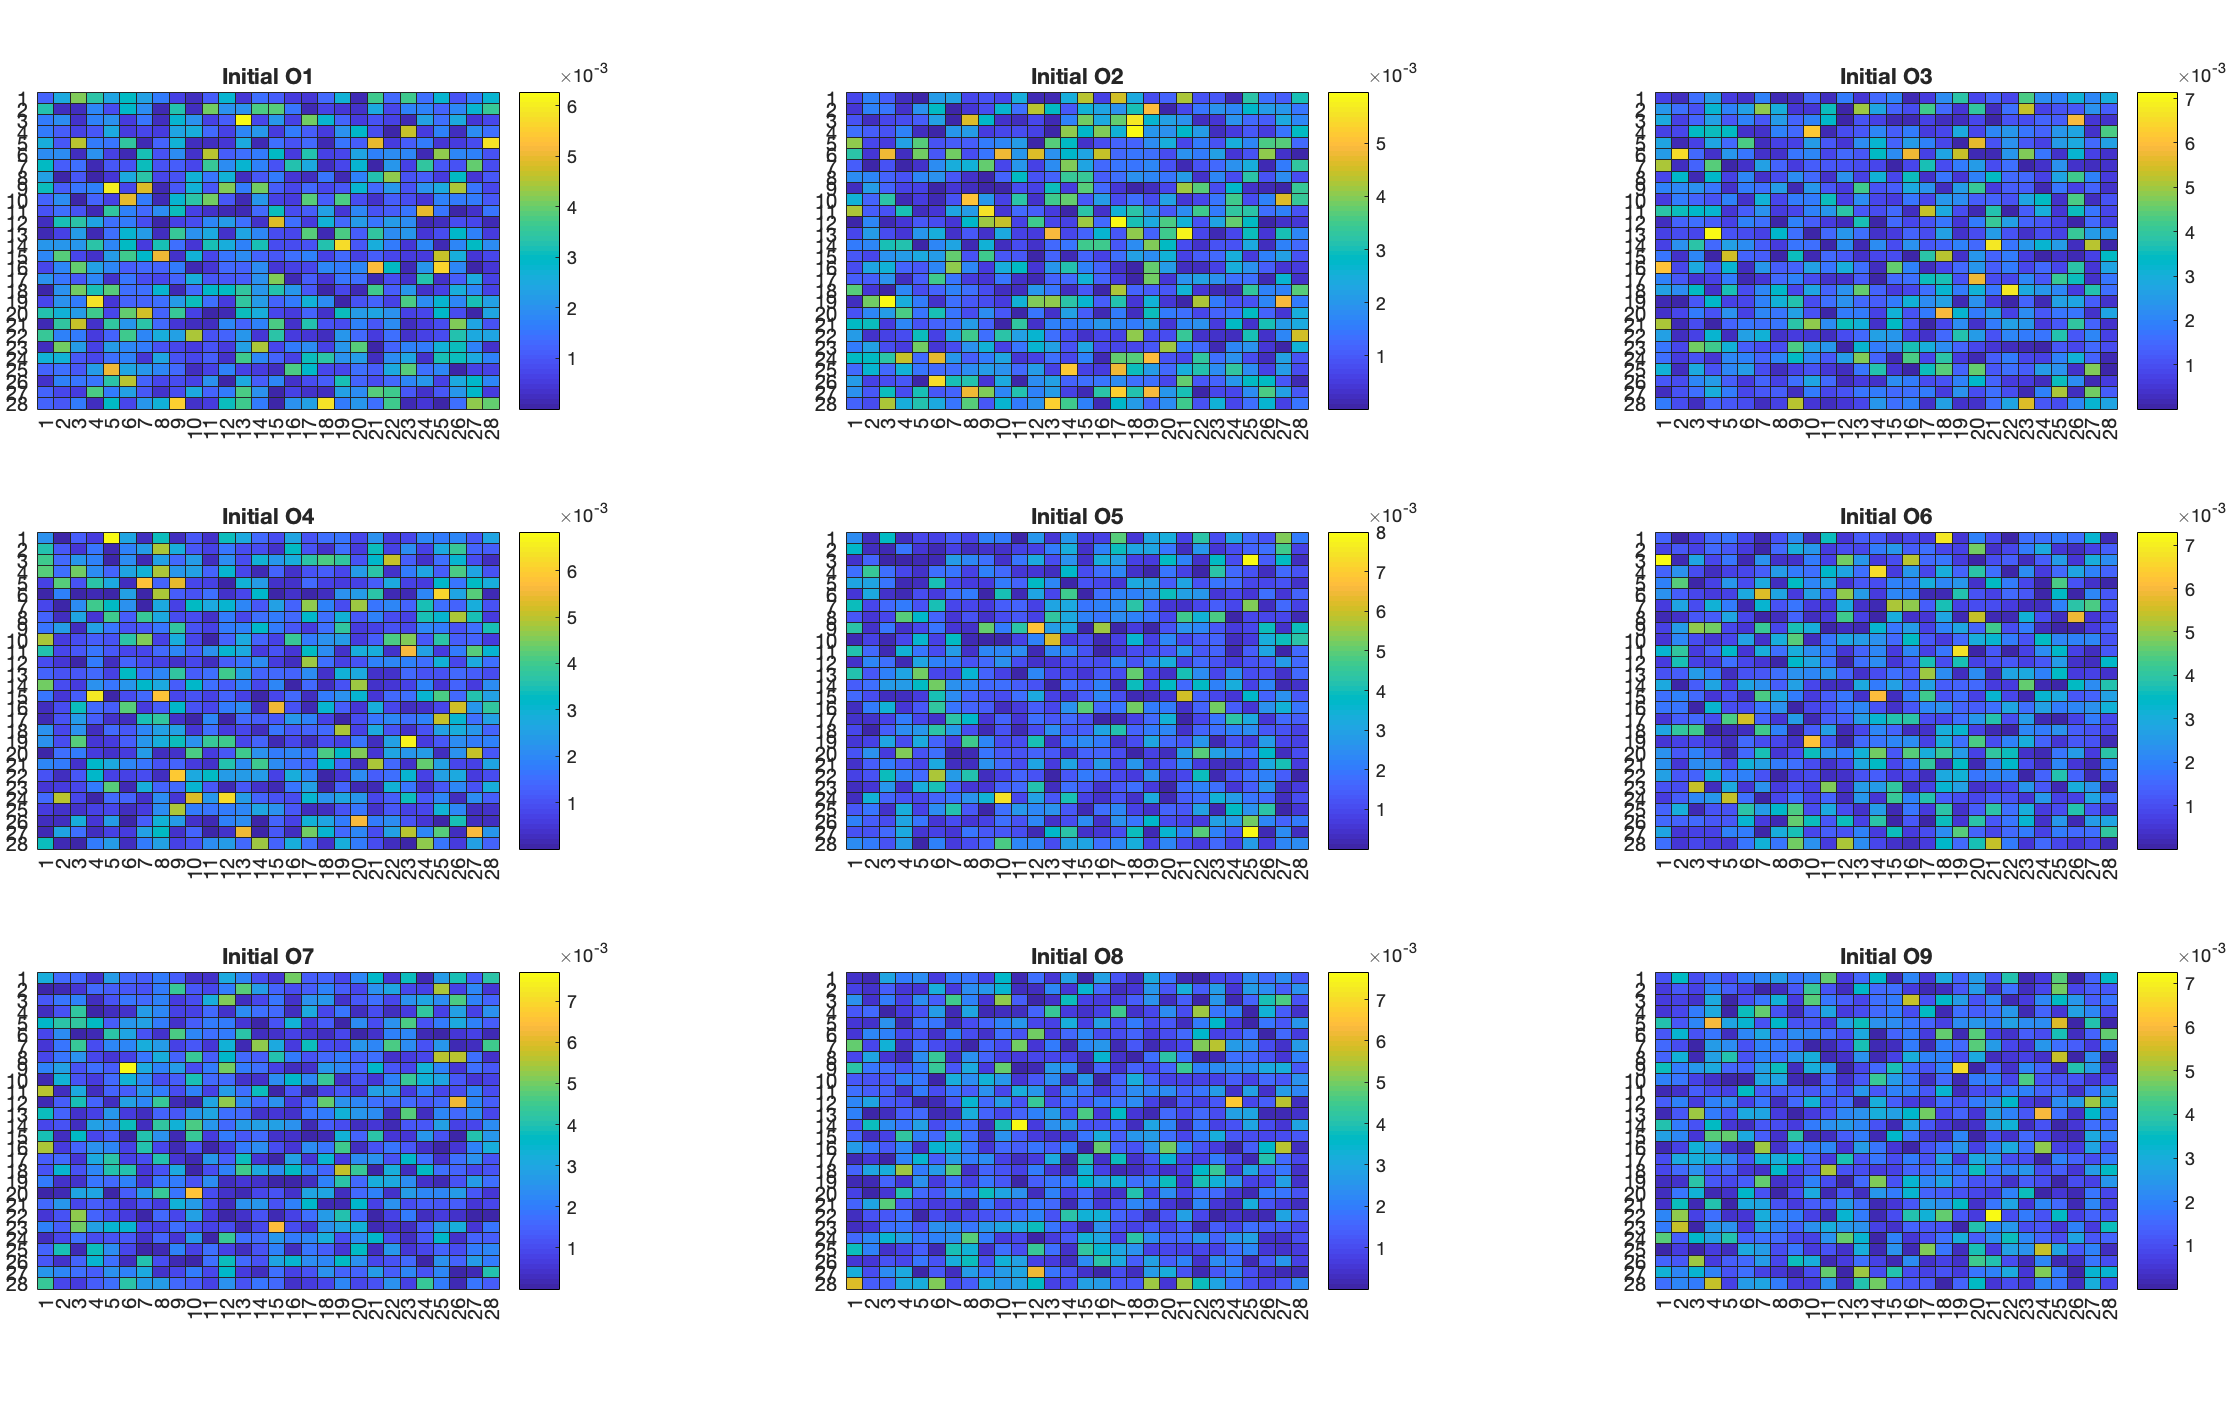
\includegraphics[width=\linewidth]{initial_synapse_weights}
	\caption{Initial Synapse Weights Heatmap}
	\label{fig:initial_synapse_weights}
\end{figure}

\begin{figure}[H]
	\centering
	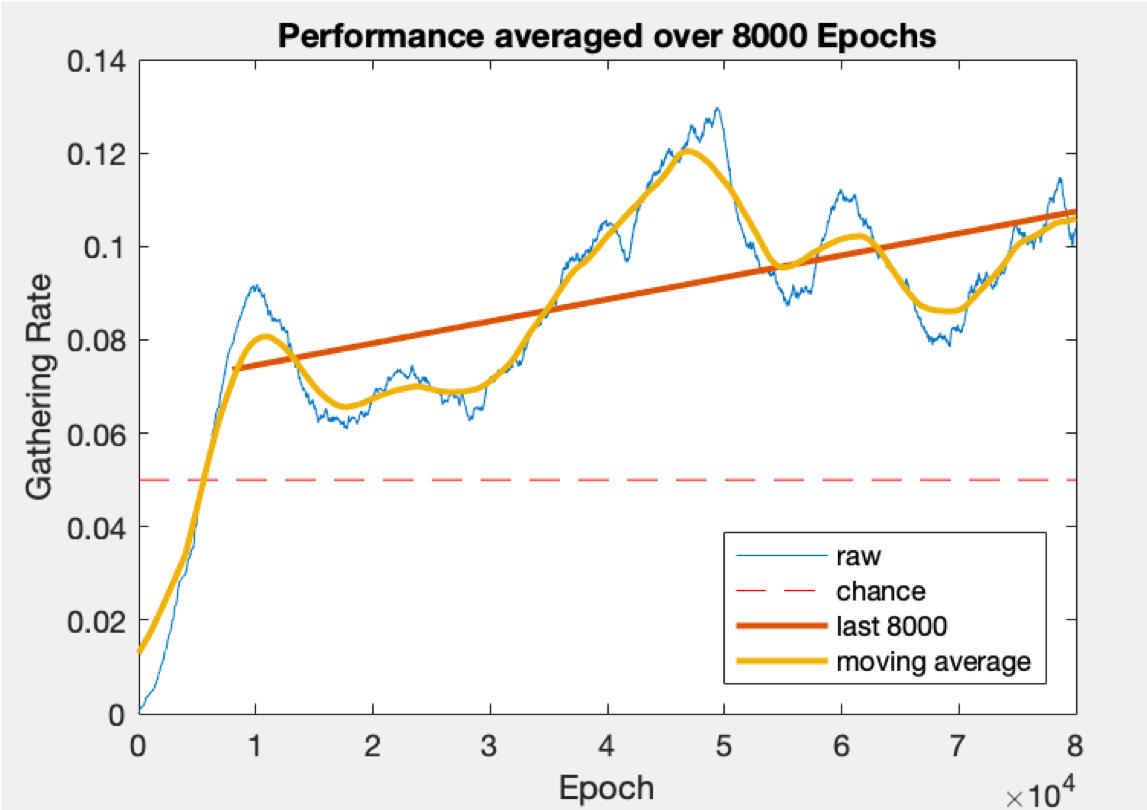
\includegraphics[width=\linewidth]{performance_improvements}
	\caption{Potential Performance Improvements 80,000 epochs starting at end of 500,000 epoch simulation but with 5 times greater soft-thresholding cap}
	\label{fig:performance_improvements}
\end{figure}

\end{document}